\documentclass{svproc}
\usepackage{graphicx} 
\usepackage{amsmath}
\usepackage{biblatex}
\addbibresource{lit.bib}

\title{Exploring the effectiveness of Small-Scale Vision and Language Models for Vision and Language Navigation Tasks in Continuous Environments}
\author{Wesley Chiu, Abdulrahman Altahhan}
\institute{University of Leeds, School of Computing, ODL MSc in AI, UK.}
\date{January 2025}

\begin{document}
\maketitle

\begin{abstract}
    Vision-and-Language Navigation (VLN) is a rapidly evolving field of research that aims to enable an embodied agent to follow textual instructions given in natural language
    to navigate through an unseen environment to a goal position. Existing approaches to this task fall into two main categories: "specialist" models that have been
    constructed and trained specifically to solve this task, and zero-shot or few-shot models that aim to leverage the implicit knowledge within Large Language Models (LLMs) and Vision 
    Language Models (VLMs). Prior work in the latter approach have used the most powerful models (70B+ parameters). This work aims to evaluate the suitability of using a lighter-weight 
    variant of an existing open-sourced model (Qwen2-VL) as the primary VLM, which would allow it to be run "on-device" rather than being connected to a broader network.
    The experiments in a simulated environment demonstrates that the current ability of the lighter-weight model is not yet fit for purpose, failing to reach the success rates 
    seen approaches that use the full-sized variants.
    
    \keywords{Vision-and-Language Navigation, Vision Language Model, Large Language Model, Prompt Engineering, Prompting}
\end{abstract}

\section{Introduction}
    This is the introduction to your project. This is nice intro. In \cite{NuclearPlant}
    
\section{Literature Review}
    \cite{TD0-Replay} has established a new TD(0) method that replays all past experiences. On the hand, \cite{TD-Replay} has taken this further to include a target that incorporates all past updates via TD($\lambda$). \cite{ConjugateTD} applied conjugate gradient update on TD.


\section{Methodology}
    In this section, we lay out the methodology. Note how in Fig. \ref{fig:my_label} we have shown the boundary.


    \begin{figure}
        \centering
        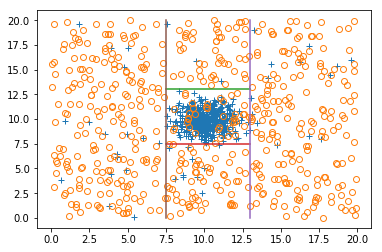
\includegraphics[scale=.75]{figures/DecisionBoundary.png}
        \caption{Caption}
        \label{fig:fig2}
    \end{figure}

    
    \begin{figure}
        \centering
        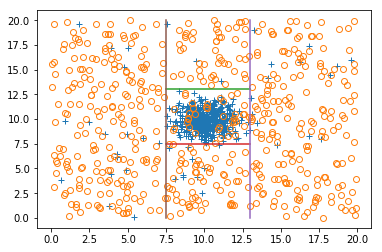
\includegraphics[scale=.75]{figures/DecisionBoundary.png}
        \caption{Caption}
        \label{fig:my_label}
    \end{figure}


    
    In Fig. \ref{fig:my_label} that $\alpha = n^2$. In eq. (\ref{eq:sum_i}) we have shown that the $ 1+2+3+4 = 4\times 5 /2=10$.
    \begin{align*}
        \sum_{i=1}^{n} y &= 10 \\
        M &= \beta ^2 \\
        \boldsymbol{B}^\top &= \boldsymbol{\Lambda}^2 \\
    \end{align*}
    
    \begin{align}
        \label{eq:sum_i}
        \sum_{i=1}^n i &= \frac{(n+1)n}{2} \\  
        \nonumber
        \beta ^2 &= \alpha_i^n
    \end{align}

\section{Experiment Results}
    \subsection{Experiment 1}
        \subsubsection{Exp}
    Note that the figure and the tables might be laid out on another page. Do not worry about that, and do not attempt to change it. Leave this to Latex.
    
    
    \begin{table}
        \caption{This is a table}
        \begin{center}
            \begin{tabular}{rlc}
                \hline
                \multicolumn{1}{l}{Year}&\multicolumn{1}{l}{World}&\multicolumn{1}{l}{Duration}\\
                \hline
                8000 B.C.  &     5,000,000 &  10\\
                  50 A.D.  &   200,000,000 &  20\\
                1650 A.D.  &   500,000,000 &  30\\
                \hline
            \end{tabular}
        \end{center}
    \end{table}

\section{Conclusion and Future Work}
We have conducted a study on ...

\printbibliography 
\end{document}
